\documentclass{article}
\usepackage{graphicx} % new way of doing eps files
\usepackage{listings} % nice code layout
\usepackage[usenames]{color} % color
\definecolor{listinggray}{gray}{0.9}
\definecolor{graphgray}{gray}{0.7}
\definecolor{ans}{rgb}{1,0,0}
\definecolor{blue}{rgb}{0,0,1}
% \Verilog{title}{label}{file}
\newcommand{\Verilog}[3]{
  \lstset{language=Verilog}
  \lstset{backgroundcolor=\color{listinggray},rulecolor=\color{blue}}
  \lstset{linewidth=\textwidth}
  \lstset{commentstyle=\textit, stringstyle=\upshape,showspaces=false}
  \lstset{frame=tb}
  \lstinputlisting[caption={#1},label={#2}]{#3}
}


\author{Steve Potter}
\title{Lab 2 - Program Counter}

\begin{document}
\maketitle

\section{Introduction}
The goal of this lab is to create an adder module and a multiplexer module.  These modules will initially be used in the Fetch stage of our 64-bit ARMv8 processor.  The adder will be used to increment the Program Counter (PC).  The incremented PC will be used for sequential program execution.  The mux will be used to set the PC to either the incremented PC or to a branch address.  This selection will be based on the mux control line, which specifies whether the program should branch or continue running sequentially.

\section{Interface}
The inputs of the adder module are a\_in and b\_in, which should be populated with the two numbers that you want to add.  The output is add\_out, which contains the sum that was produced in the adder module.

The inputs of the mux are a\_in, b\_in, and control.  a\_in and b\_in are the two signals that are available to be selected, and control is the signal that is used to select whether the value of a\_in or b\_in will be chosen by the mux.  The output of the mux is mux\_out, which contains the value that the mux selected.

\section{Design}
The first module to build is the adder module.  The adder module is designed to take two 64-bit input values and produce a 64-bit sum as an output.

The second module to build is the mux module.  The mux module is designed to take two input values and select one of the two inputs to connect to the output line.  This selection is done by evaluating the control line.  If the control line is 0, then the mux should output the value of a\_in.  If the control line is 1, then the mux should output the value of b\_in.  The size of the a\_in, b\_in, and mux\_out can be assigned when the module is instantiated, allowing this module to be used for signals of any size.

\section{Implementation}
The adder module is implemented by adding a\_in + b\_in and assigning the sum to add\_out.  This is done with a continuous assignment because we are using combinational logic, where the output should be constantly evaluated and update immediately when inputs change.  View the adder code in Listing~\ref{code:adder} on page~\pageref{code:adder}.

\Verilog{Verilog code for implementing an adder.}{code:adder}{../code/0_common/adder.v}

The mux module is implemented using the conditional operator (?).  If the control signal is 1, then mux\_out is set to b\_in.  If the control signal is 1, then mux\_out is set to a\_in.  Note that this operation is done in a continuous assign statement.  The continuous assignment is used because we need combinational logic, where the output should be constantly evaluated and update immediately when inputs change.  

The other interesting aspect of the implementation is the use of the SIZE parameter.  The SIZE parameter allows the user of the module to specify the SIZE when instantiating the module, which allows this module to be used as a mux of any size.  To utilize this feature to instantiate a 64-bit mux, you would instantiate it as mux\#(64) UUT.  If you do not specify a size, the default value of 8 will be used.  View the mux code in Listing~\ref{code:mux} on page~\pageref{code:mux}.  

\Verilog{Verilog code for implementing a mux.}{code:mux}{../code/0_common/mux.v}

\section{Test Bench Design}
The adder test bench creates regs for a and b as well as a wire for the add\_out output of the adder module.  All signals are 64-bits.  An adder module, UUT, is instantiated, and then a series of a and b inputs are set in the initial section.  Regs a and b are set using non-blocking procedural assignments, then a cycle delay is initiated.  As defined in definitions.vh, a cycle is 10ns.  Then a and b are changed several times, with various amounts of delay.  The goal is to test a variety of inputs and outputs at various intervals.  The results of the test are verified by evaluating the simulation results and verifying that add\_out equals a + b at all times.  View the adder\_test code in Listing~\ref{code:addertest} on page~\pageref{code:addertest}.

\Verilog{Verilog code for testing the adder.}{code:addertest}{../code/0_common/adder_test.v}


The mux test bench creates regs for a, b, and control as well as a wire for the mux\_out output of the mux module.  All signals are 64-bits.  An adder module, UUT, is instantiated with a size of 64 by using the syntax of mux\#(64) UUT.  Then a series of a and b inputs are set in the initial section, and the control line is set to 0.  a and b are varied with various amounts of delay.  After several cycles, control is changed to 1, causing the value of b to be sent to mux\_out.  And then control is set back to 0 to verify that the mux can switch back and forth effectively.  The results of the test are verified by evaluating the simulation results and verifying that:
\begin{enumerate}
	\item mux\_out always equals a when control is 0 
	\item mux\_out always equals b when control is 1
\end{enumerate} 
View the mux\_test code in Listing~\ref{code:muxtest} on page~\pageref{code:muxtest}.

\Verilog{Verilog code for testing the mux.}{code:muxtest}{../code/0_common/mux_test.v}

\section{Simulation}
The Simulation Results of the adder test confirm that the adder works as expected, with add\_out always producing the sum of a and b.  The timing diagram can be viewed in Figure~\ref{fig:addertest} on page~\pageref{fig:addertest}.

The Simulation Results of the mux test confirm that the mux works as expected, with mux\_out always matching the conditions listed in the Test Bench Design section.  The timing diagram can be viewed in Figure~\ref{fig:muxtest} on page~\pageref{fig:muxtest}.

\begin{figure}
\begin{center}
\caption{Timing diagram for the adder test.}\label{fig:addertest}
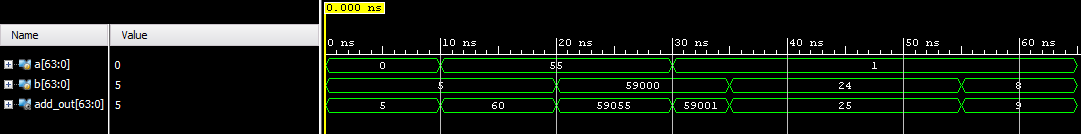
\includegraphics[width=0.9\textwidth]{../images/adder_test.png}
\end{center}
\end{figure}

\begin{figure}
	\begin{center}
		\caption{Timing diagram for the mux test.}\label{fig:muxtest}
		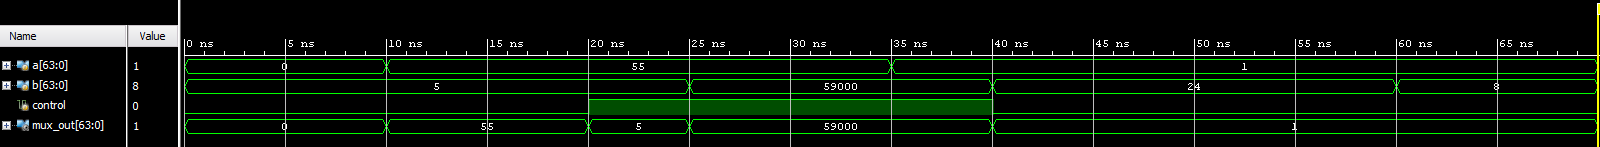
\includegraphics[width=0.9\textwidth]{../images/mux_test.png}
	\end{center}
\end{figure}

\section{Conclusions}
An adder module and mux module were successfully created.  The adder module can be used in the Fetch stage to increment the PC, and it can be used any other place that 64-bit numbers need to be added.  The mux module can now be used in the Fetch stage to select between the incremented PC and the branch target address.  Since it was designed with a SIZE parameter, it can be used to instantiate a mux for any data size.  While the Fetch stage will use a 64-bit mux, this flexibility will be useful in future stages.
\end{document} 